% Options for packages loaded elsewhere
\PassOptionsToPackage{unicode}{hyperref}
\PassOptionsToPackage{hyphens}{url}
\PassOptionsToPackage{dvipsnames,svgnames,x11names}{xcolor}
%
\documentclass[
  letterpaper,
  DIV=11,
  numbers=noendperiod]{scrartcl}

\usepackage{amsmath,amssymb}
\usepackage{lmodern}
\usepackage{iftex}
\ifPDFTeX
  \usepackage[T1]{fontenc}
  \usepackage[utf8]{inputenc}
  \usepackage{textcomp} % provide euro and other symbols
\else % if luatex or xetex
  \usepackage{unicode-math}
  \defaultfontfeatures{Scale=MatchLowercase}
  \defaultfontfeatures[\rmfamily]{Ligatures=TeX,Scale=1}
\fi
% Use upquote if available, for straight quotes in verbatim environments
\IfFileExists{upquote.sty}{\usepackage{upquote}}{}
\IfFileExists{microtype.sty}{% use microtype if available
  \usepackage[]{microtype}
  \UseMicrotypeSet[protrusion]{basicmath} % disable protrusion for tt fonts
}{}
\makeatletter
\@ifundefined{KOMAClassName}{% if non-KOMA class
  \IfFileExists{parskip.sty}{%
    \usepackage{parskip}
  }{% else
    \setlength{\parindent}{0pt}
    \setlength{\parskip}{6pt plus 2pt minus 1pt}}
}{% if KOMA class
  \KOMAoptions{parskip=half}}
\makeatother
\usepackage{xcolor}
\usepackage[normalem]{ulem}
\setlength{\emergencystretch}{3em} % prevent overfull lines
\setcounter{secnumdepth}{-\maxdimen} % remove section numbering
% Make \paragraph and \subparagraph free-standing
\ifx\paragraph\undefined\else
  \let\oldparagraph\paragraph
  \renewcommand{\paragraph}[1]{\oldparagraph{#1}\mbox{}}
\fi
\ifx\subparagraph\undefined\else
  \let\oldsubparagraph\subparagraph
  \renewcommand{\subparagraph}[1]{\oldsubparagraph{#1}\mbox{}}
\fi


\providecommand{\tightlist}{%
  \setlength{\itemsep}{0pt}\setlength{\parskip}{0pt}}\usepackage{longtable,booktabs,array}
\usepackage{calc} % for calculating minipage widths
% Correct order of tables after \paragraph or \subparagraph
\usepackage{etoolbox}
\makeatletter
\patchcmd\longtable{\par}{\if@noskipsec\mbox{}\fi\par}{}{}
\makeatother
% Allow footnotes in longtable head/foot
\IfFileExists{footnotehyper.sty}{\usepackage{footnotehyper}}{\usepackage{footnote}}
\makesavenoteenv{longtable}
\usepackage{graphicx}
\makeatletter
\def\maxwidth{\ifdim\Gin@nat@width>\linewidth\linewidth\else\Gin@nat@width\fi}
\def\maxheight{\ifdim\Gin@nat@height>\textheight\textheight\else\Gin@nat@height\fi}
\makeatother
% Scale images if necessary, so that they will not overflow the page
% margins by default, and it is still possible to overwrite the defaults
% using explicit options in \includegraphics[width, height, ...]{}
\setkeys{Gin}{width=\maxwidth,height=\maxheight,keepaspectratio}
% Set default figure placement to htbp
\makeatletter
\def\fps@figure{htbp}
\makeatother
\newlength{\cslhangindent}
\setlength{\cslhangindent}{1.5em}
\newlength{\csllabelwidth}
\setlength{\csllabelwidth}{3em}
\newlength{\cslentryspacingunit} % times entry-spacing
\setlength{\cslentryspacingunit}{\parskip}
\newenvironment{CSLReferences}[2] % #1 hanging-ident, #2 entry spacing
 {% don't indent paragraphs
  \setlength{\parindent}{0pt}
  % turn on hanging indent if param 1 is 1
  \ifodd #1
  \let\oldpar\par
  \def\par{\hangindent=\cslhangindent\oldpar}
  \fi
  % set entry spacing
  \setlength{\parskip}{#2\cslentryspacingunit}
 }%
 {}
\usepackage{calc}
\newcommand{\CSLBlock}[1]{#1\hfill\break}
\newcommand{\CSLLeftMargin}[1]{\parbox[t]{\csllabelwidth}{#1}}
\newcommand{\CSLRightInline}[1]{\parbox[t]{\linewidth - \csllabelwidth}{#1}\break}
\newcommand{\CSLIndent}[1]{\hspace{\cslhangindent}#1}

\KOMAoption{captions}{tableheading}
\makeatletter
\makeatother
\makeatletter
\makeatother
\makeatletter
\@ifpackageloaded{caption}{}{\usepackage{caption}}
\AtBeginDocument{%
\ifdefined\contentsname
  \renewcommand*\contentsname{Table of contents}
\else
  \newcommand\contentsname{Table of contents}
\fi
\ifdefined\listfigurename
  \renewcommand*\listfigurename{List of Figures}
\else
  \newcommand\listfigurename{List of Figures}
\fi
\ifdefined\listtablename
  \renewcommand*\listtablename{List of Tables}
\else
  \newcommand\listtablename{List of Tables}
\fi
\ifdefined\figurename
  \renewcommand*\figurename{Figure}
\else
  \newcommand\figurename{Figure}
\fi
\ifdefined\tablename
  \renewcommand*\tablename{Table}
\else
  \newcommand\tablename{Table}
\fi
}
\@ifpackageloaded{float}{}{\usepackage{float}}
\floatstyle{ruled}
\@ifundefined{c@chapter}{\newfloat{codelisting}{h}{lop}}{\newfloat{codelisting}{h}{lop}[chapter]}
\floatname{codelisting}{Listing}
\newcommand*\listoflistings{\listof{codelisting}{List of Listings}}
\makeatother
\makeatletter
\@ifpackageloaded{caption}{}{\usepackage{caption}}
\@ifpackageloaded{subcaption}{}{\usepackage{subcaption}}
\makeatother
\makeatletter
\@ifpackageloaded{tcolorbox}{}{\usepackage[many]{tcolorbox}}
\makeatother
\makeatletter
\@ifundefined{shadecolor}{\definecolor{shadecolor}{rgb}{.97, .97, .97}}
\makeatother
\makeatletter
\makeatother
\ifLuaTeX
  \usepackage{selnolig}  % disable illegal ligatures
\fi
\IfFileExists{bookmark.sty}{\usepackage{bookmark}}{\usepackage{hyperref}}
\IfFileExists{xurl.sty}{\usepackage{xurl}}{} % add URL line breaks if available
\urlstyle{same} % disable monospaced font for URLs
\hypersetup{
  pdftitle={ML/AI in CNC and machining},
  colorlinks=true,
  linkcolor={blue},
  filecolor={Maroon},
  citecolor={Blue},
  urlcolor={Blue},
  pdfcreator={LaTeX via pandoc}}

\title{ML/AI in CNC and machining}
\author{}
\date{1/7/23}

\begin{document}
\maketitle
\ifdefined\Shaded\renewenvironment{Shaded}{\begin{tcolorbox}[boxrule=0pt, interior hidden, sharp corners, frame hidden, borderline west={3pt}{0pt}{shadecolor}, enhanced, breakable]}{\end{tcolorbox}}\fi

\renewcommand*\contentsname{Table of contents}
{
\hypersetup{linkcolor=}
\setcounter{tocdepth}{3}
\tableofcontents
}
\hypertarget{review-papers}{%
\subsection{Review papers}\label{review-papers}}

\hypertarget{bertolini2021}{%
\subsubsection{Bertolini2021}\label{bertolini2021}}

\textbf{Machine Learning for industrial applications: A comprehensive
literature review}

\(5/5 \star\)

\begin{quote}
Article (Bertolini2021)\\
Bertolini, M.; Mezzogori, D.; Neroni, M. \& Zammori, F.\\
Machine Learning for industrial applications: A comprehensive literature
review Expert Systems with Applications, 2021, 175, 114820
\end{quote}

\begin{itemize}
\item
  Good review paper, classifies papers by Application Domain and by ML
  algorithm.
\item
  Not only for CNC / machining, but many types of industrial
  applications
\item
  Large number of papers surveyed
\item
  Hot and not-so-hot topics, clustered:

  \begin{quote}
  Using these metrics, five main clusters can be identified. These are:

  \begin{enumerate}
  \def\labelenumi{\arabic{enumi}.}
  \tightlist
  \item
    \textbf{Question Marks (Low Age and Negative Trend)} -- Recently
    introduced topics, that have not got a follow-up, yet. Thermography
    (THER), Cyber-Physical Systems (CPS), and Design For (D4) belong to
    this category.
  \item
    \textbf{Hot Topics (Low Age and \sout{Negative} Positive Trend)} --
    Very recent topics of booming interest. At present, none of the
    keywords properly belong to this category. Yet, Additive
    Manufacturing (ADD\_MN), Prediction \& Prognostic (PR\_PR), and
    Industry 4.0 (I4.0) are those who come closest to this category. For
    this reason, they have been labeled as `new promises'.
  \item
    \textbf{Consolidated (Medium Age and Stable Trend)} -- Not recent
    topics, which are still studied, but without the initial spike of
    interests. Topics such as Supply Chain Management (SCMI), Flexible
    Manufacturing Systems (FMS), Inventory Control (INV\_CTRI), and Tool
    Monitoring (TLL\_MN) belong to this category.
  \item
    \textbf{Stars (High Age and Positive Trend)} -- Old and consolidated
    topics that are still attracting increasing research interest.
    Topics such as Diagnosis and Fault Detection (DG\_FLT),
    Manufacturing Process (MN\_PR), Intelligent Manufacturing (INT\_MN),
    and Big Data analysis (BD\_DM) certainly belong to this class.
    Probably, Simulation (SIM) and the Internet of Things (IoT) are on
    their way to become stars.
  \item
    \textbf{Obsoletes (High Age and Negative Trend)} -- Old topics that
    have never received much scientific interest and that have almost
    disappeared from the technical literature. Due to the recent
    introduction of ML, for operation management, no keywords can be
    classified as obso­ letes yet. However, Order Management (OM) and,
    probably, also Feature Extraction (FT\_EX) are moving toward this
    class.
  \end{enumerate}
  \end{quote}

  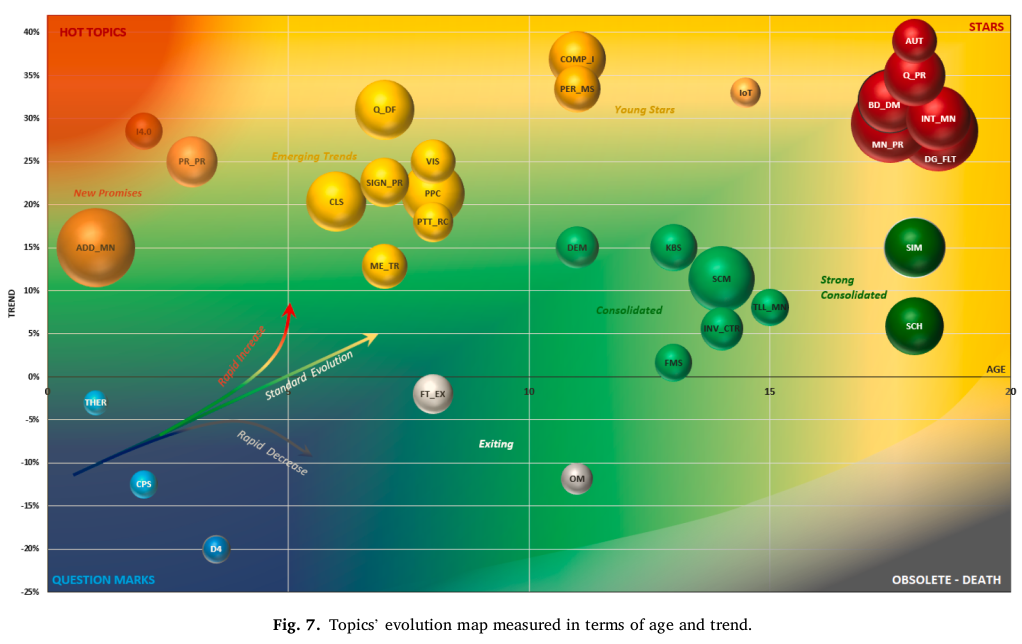
\includegraphics{img/2023-01-07-12-44-41.png}
\end{itemize}

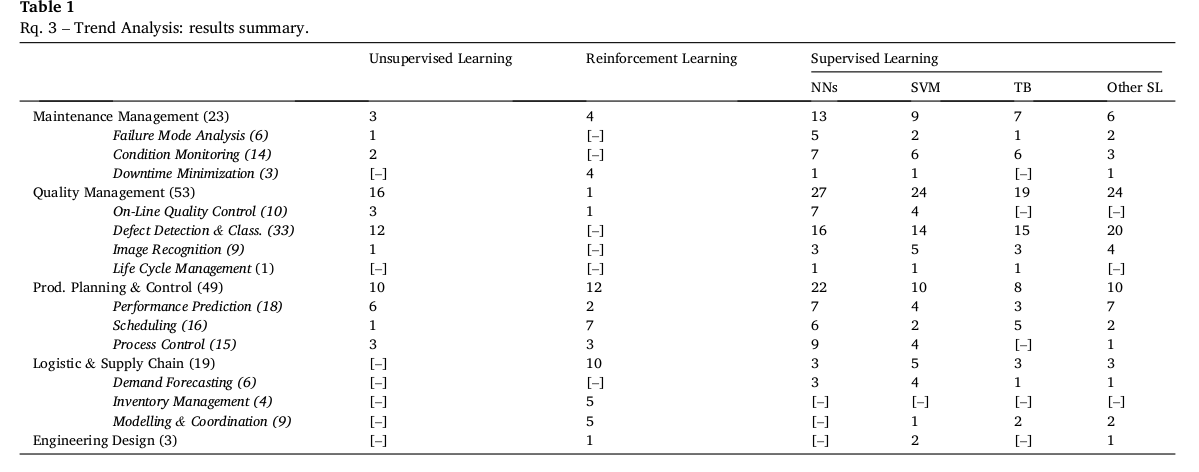
\includegraphics{img/2023-01-07-12-32-41.png}

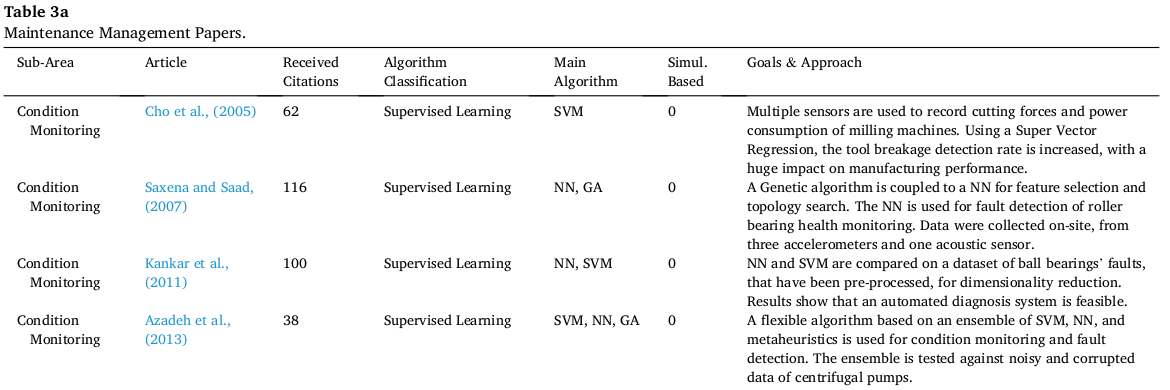
\includegraphics{img/2023-01-07-12-38-32.png} \ldots{}

\begin{itemize}
\item
  Anomaly detection examples:

  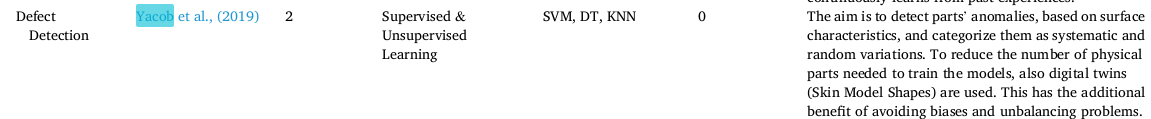
\includegraphics{img/2023-01-07-12-48-20.png}

  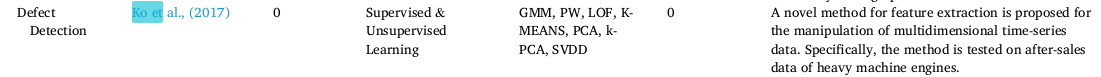
\includegraphics{img/2023-01-07-12-49-39.png}
\item
  Sample variables commonly used in datasets:

  \begin{quote}
  Table 4, which provides some indications concerning the variables that
  are commonly used per each application domain and sub-area
  \end{quote}

  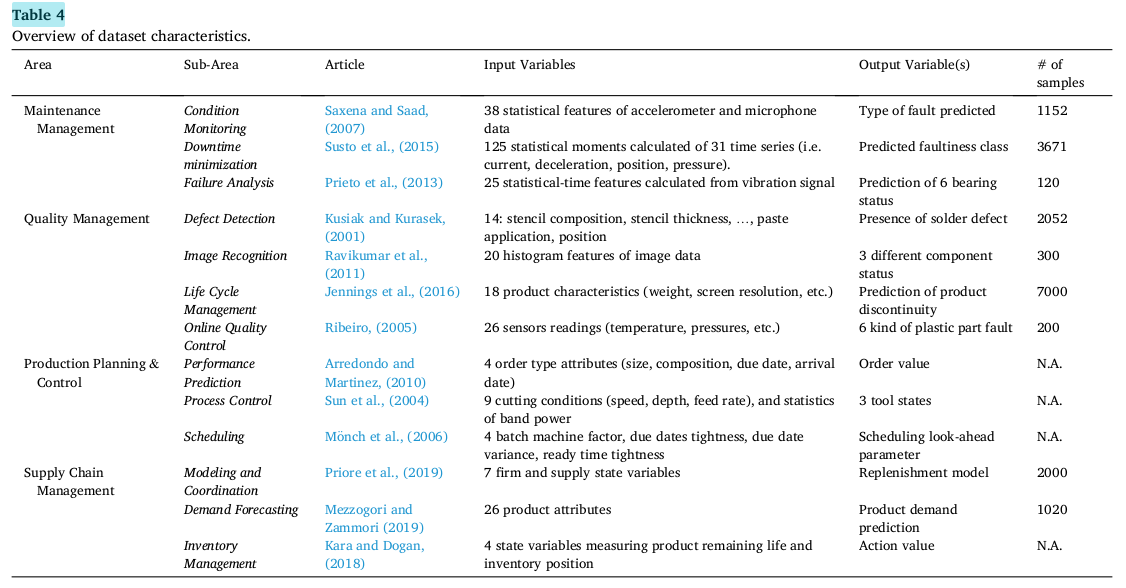
\includegraphics{img/2023-01-07-12-53-08.png}
\end{itemize}

\hypertarget{interesting-aspects}{%
\paragraph{Interesting aspects}\label{interesting-aspects}}

\begin{enumerate}
\def\labelenumi{\arabic{enumi}.}
\tightlist
\item
  Maintenance management: keep assets and machines at a full operating
  state

  \begin{itemize}
  \tightlist
  \item
    Failure Mode Analysis: Faults detection and classification. Easily
    interpreted as a prediction task, where historical data are
    collected on the production floor, and faulty and non-faulty events
    are used as ground-truth data against which a prediction model can
    be trained (NN, SVM)
  \item
    Condition Monitoring: the most common applications concern condition
    monitoring of rotating mechanical systems and rolling bearings. The
    problem is solved using vibrations and/or acoustic signals as
    classifiers inputs.
  \item
    Downtime Minimization: Plan predictive maintainance operations
    smartly, to minimize costs.
  \end{itemize}
\item
  Quality Management

  \begin{itemize}
  \tightlist
  \item
    Defects' Detection and Classification

    \begin{itemize}
    \tightlist
    \item
      Unbalanced datasets
    \end{itemize}
  \item
    Visual quality inspection: detect defects by image classification
  \end{itemize}
\item
  Production Planning \& Control (PPC)

  \begin{itemize}
  \tightlist
  \item
    Performance Prediction and Optimization: order acceptance policy,
    optimal sequence of technical steps, reduce electricity consumption,
    optimize parameters
  \item
    Scheduling: NP-hard, select dispatching rules, dynamic scheduling
    based on conditions
  \item
    Process Control: Reinforcement Learning to automate a process;
    optimizing parameters for safe behavior in non-conforming
    operations.
  \end{itemize}
\item
  Supply Chain Management: logistics

  \begin{itemize}
  \tightlist
  \item
    Modeling and Coordination: Reinforcement Learning
  \item
    Demand Forecasts: prediction models
  \item
    Inventory Control:\\
  \item
    complex modeling of supply chains, not easy, RL is a good fit here
  \end{itemize}
\end{enumerate}

Other things: - noisy data is common, many techniques used to clean it -
unbalanced data - low interpretability, with Deep NNs

\begin{center}\rule{0.5\linewidth}{0.5pt}\end{center}

\hypertarget{kim2018}{%
\subsubsection{Kim2018}\label{kim2018}}

\textbf{Smart Machining Process Using Machine Learning: A Review and
Perspective on Machining Industry (2018) (Kim et al. 2018)}

\(3/5 \star\)

Contains a listing of many machining problems where machine learning
algorithms have been used in machining.

\begin{itemize}
\tightlist
\item
  Machine processes: General, milling, drilling
\item
  Purpose: Tool wear and breakage, predict energy consumption, surface
  roughness prediction, process parameter optimization
\item
  Algorithms: SVM and SVR, various NNs, Random forests, linear
  regression, k-NN, depending on task
\end{itemize}

\begin{center}\rule{0.5\linewidth}{0.5pt}\end{center}

\hypertarget{tambake2021}{%
\subsubsection{Tambake2021}\label{tambake2021}}

\textbf{Data Driven Cutting Tool Fault Diagnosis System Using Machine
Learning Approach: A Review (Tambake, Deshmukh, and Patange 2021)}

\(2/5 \star\)

\begin{itemize}
\tightlist
\item
  Poorly written, but contains a list of papers on fault detection
\end{itemize}

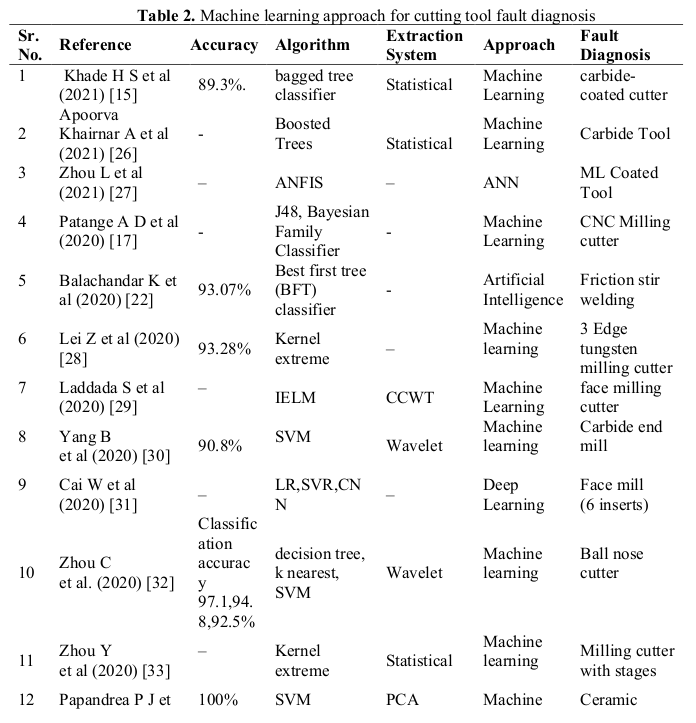
\includegraphics{img/2023-01-07-12-19-30.png}

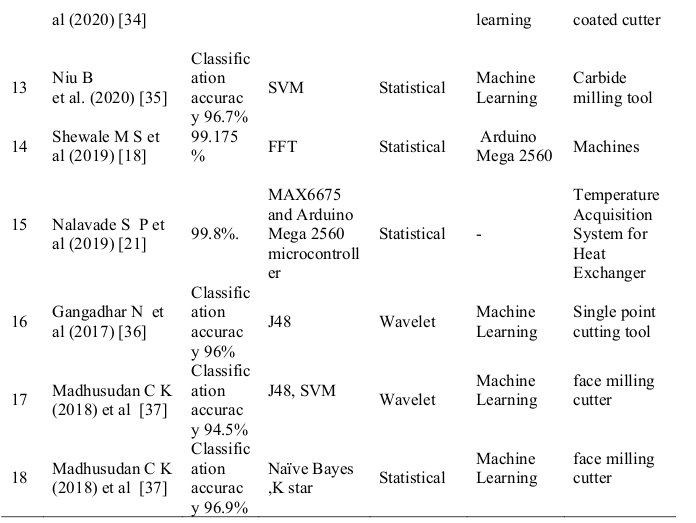
\includegraphics{img/2023-01-07-12-20-27.png}

\begin{center}\rule{0.5\linewidth}{0.5pt}\end{center}

\hypertarget{technical-papers}{%
\subsection{Technical papers}\label{technical-papers}}

\hypertarget{ordas2017}{%
\subsubsection{Ordas2017}\label{ordas2017}}

\textbf{Wear Characterization of the Cutting Tool in Milling Processes
using Shape and Texture Descriptors (PhD thesis, 2017)(García-Ordás
2017)}

\begin{itemize}
\item
  PhD thesis which proposes and evaluates some image-based descriptors
  to characterize tool wear, using a cheap Raspberry Pi + camera setup
  which captures images of the cutting tool.
\item
  Investigative / no remarkable results.
\end{itemize}

\begin{center}\rule{0.5\linewidth}{0.5pt}\end{center}

\hypertarget{papandrea2020}{%
\subsubsection{Papandrea2020}\label{papandrea2020}}

\textbf{Surface roughness diagnosis in hard turning using acoustic
signals and support vector machine: A PCA-based approach (Papandrea et
al. 2020)}

\begin{itemize}
\tightlist
\item
  Supervised Learning
\item
  Surface roughness classification, based on acoustic signals during
  cutting.
\item
  Use STFT followed by PCA per coefficients, and SVM for classification.
\item
  Tested on CNC, with stock microphone
\item
  Some complicated experimental machining setups, several parameters in
  the process (rotating speed, feed rate). The experimental setups
  depend on many factors.
\item
  Results weak. Some PCA coeffs are correlated with roughness, and can
  be clustered consistently into 3 groups, which can then be identified
  in test sets.
\item
  More investigative / basic research, no remarkable results.
\end{itemize}

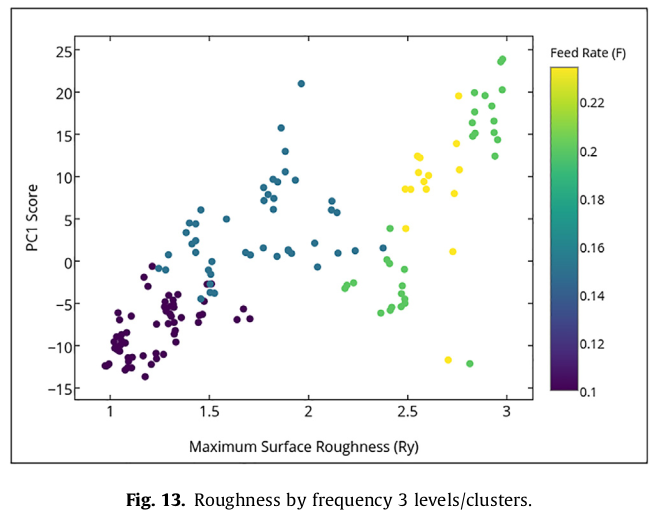
\includegraphics{img/2023-01-07-12-16-33.png}

\begin{center}\rule{0.5\linewidth}{0.5pt}\end{center}

\hypertarget{cho2005}{%
\subsubsection{Cho2005}\label{cho2005}}

\textbf{Tool breakage detection using support vector machine learning in
a milling process (Cho et al. 2005)}

\begin{quote}
Article (Cho2005)\\
Cho, S.; Asfour, S.; Onar, A. \& Kaundinya, N.\\
Tool breakage detection using support vector machine learning in a
milling process\\
International Journal of Machine Tools and Manufacture, 2005, 45,
241-249
\end{quote}

\begin{itemize}
\tightlist
\item
  Supervised Learning
\item
  Detect two types of tool breakage: shank breakage and flute breakage
\item
  Cutting forces + power consumption (proportional with force) +
  SVRegression =\textgreater{} detect flute breakage
\item
  Idea:

  \begin{itemize}
  \tightlist
  \item
    In normal operation, model the cutting force / normal power
    consumption based on spindle speed, feed rate, depth of cut with
    SVRegression (alternative: with multiple linear regression)
  \item
    Detection: if actual measured values deviate a lot from model
    predictions (by a threshold), we have a breakage.
  \end{itemize}
\item
  SVR is hard to parameterize!
\end{itemize}

\begin{center}\rule{0.5\linewidth}{0.5pt}\end{center}

\hypertarget{li2017}{%
\subsubsection{Li2017}\label{li2017}}

\textbf{An Ensemble Deep Convolutional Neural Network Model with
Improved D-S Evidence Fusion for Bearing Fault Diagnosis (Li et al.
2017)}

\begin{quote}
Article (Li2017)\\
Li, S.; Liu, G.; Tang, X.; Lu, J. \& Hu, J.\\
An Ensemble Deep Convolutional Neural Network Model with Improved D-S
Evidence Fusion for Bearing Fault Diagnosis\\
Sensors, Multidisciplinary Digital Publishing Institute, 2017, 17, 1729
\end{quote}

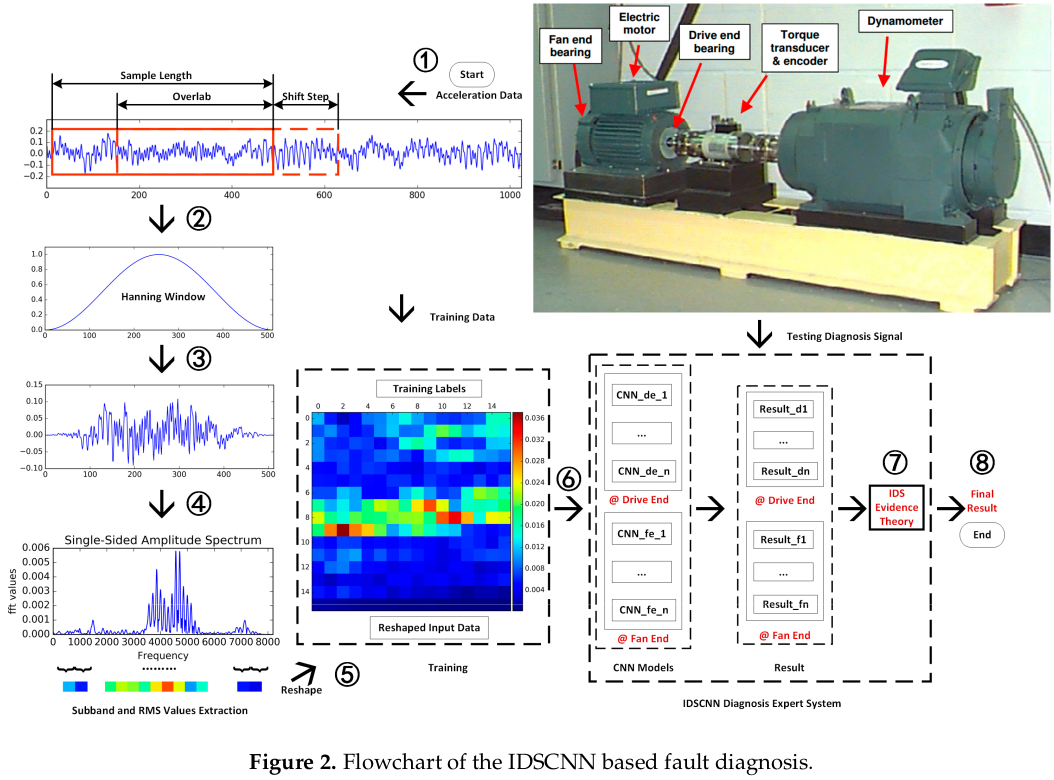
\includegraphics{img/2023-01-08-19-37-45.png}

\begin{itemize}
\tightlist
\item
  Supervised Learning
\item
  For bearing fault detection, with deep neural networks
\item
  Using Dempster--Shafer (D-S) evidence theory for sensor fusion,
  improves it with custom modifications
\item
  Raw signals: acceleration and vibration from 2 sensors
\item
  Data preprocessing: sliding windows, subband, RMS, reshape to square
  images
\item
  Small CNN trained in images, used as feature extractors
\item
  CNN outputs are fused with the Improved D-S scheme
\end{itemize}

\begin{center}\rule{0.5\linewidth}{0.5pt}\end{center}

\hypertarget{kankar2011}{%
\subsubsection{Kankar2011}\label{kankar2011}}

\textbf{Fault diagnosis of ball bearings using machine learning methods
(Kankar, Sharma, and Harsha 2011)}

\begin{quote}
Article (Kankar2011)\\
Kankar, P. K.; Sharma, S. C. \& Harsha, S. P.\\
Fault diagnosis of ball bearings using machine learning methods\\
Expert Systems with Applications, 2011, 38, 1876-1886
\end{quote}

\begin{itemize}
\item
  Supervised Learning
\item
  Detect defects and in ball bearings based on vibration data collected
  with accelerometers
\item
  2D acceleration signals (horizontal and vertical)
\item
  Recording length = about 0.5 to 1 second
\item
  5 classes:

  \begin{itemize}
  \tightlist
  \item
    Healthy bearings (HB).
  \item
    Bearing with outer race crack (BORC).
  \item
    Bearing with rough inner race surface (BRIR).
  \item
    Ball with corrosion pitting (BCP).
  \item
    Combined bearing component defects (CBD)
  \end{itemize}
\item
  \textbf{Manual features} (range, mean, kurtosis etc):

  6 features from horizontal + 6 features vertical + speed + ``number of
  loader'' =\textless{} 14 features per instance
\item
  Feature selection step (not clear how)
\item
  Results: accuracy about 70\%
\end{itemize}

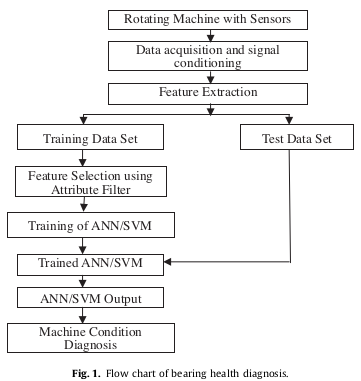
\includegraphics{img/2023-01-09-12-28-36.png}

\begin{center}\rule{0.5\linewidth}{0.5pt}\end{center}

\hypertarget{ong2019}{%
\subsubsection{Ong2019}\label{ong2019}}

\textbf{Tool condition monitoring in CNC end milling using wavelet
neural network based on machine vision (Ong, Lee, and Lau 2019)}

\begin{quote}
Article (Ong2019)\\
Ong, P.; Lee, W. K. \& Lau, R. J. H.\\
Tool condition monitoring in CNC end milling using wavelet neural
network based on machine vision\\
The International Journal of Advanced Manufacturing Technology, 2019,
104, 1369-1379
\end{quote}

\begin{itemize}
\item
  Nice introduction and review:

  \begin{itemize}
  \item
    \begin{quote}
    For the indirect method of tool condition monitoring, there are
    considerably numerous studies attempting to correlate the
    relationship between the machining parameters with tool wear
    \end{quote}
  \item
    tool wear detection with visual and non-visual signals (cutting
    force, sound, vibration)
  \item
    tool wear estimation by visually analyzing the surface of the
    machined part
  \end{itemize}
\item
  Ue a special type of NN, Wavelet Neural Network, to predict
  \textbf{flank wear}. WNN is just their quirk.
\item
  WNN are a generalized form of RBF-NN, with wavelet activation
  functions
\item
  Use images of the tool itself and/or the surface of the machined part
\item
  Image preprocessing of the worn region of the tool:

  \includegraphics{.pdf}img/2023-01-09-12-54-18.png
\item
  NN architecture used. Shallow with 1 hidden layer:

  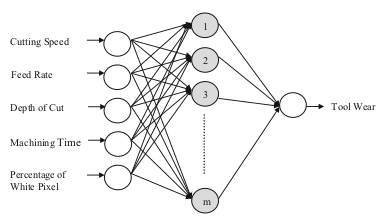
\includegraphics{img/2023-01-09-12-55-14.png}
\item
  Dataset: just 126 images
\item
  Results: good predictions by pretty much all methods compared.

  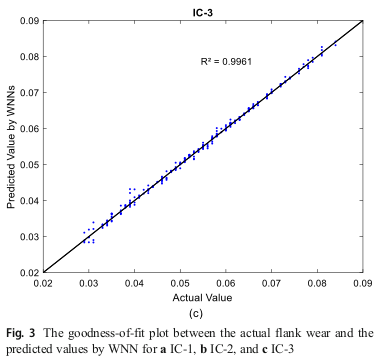
\includegraphics{img/2023-01-09-13-01-36.png}
\end{itemize}

\begin{center}\rule{0.5\linewidth}{0.5pt}\end{center}

\hypertarget{hahn2021}{%
\subsubsection{Hahn2021}\label{hahn2021}}

\begin{quote}
Article (Hahn2021)\\
Hahn, T. V. \& Mechefske, C. K.\\
Self-supervised learning for tool wear monitoring with a
disentangled-variational-autoencoder\\
International Journal of Hydromechatronics, Inderscience Publishers,
2021, 4, 69-98
\end{quote}

\begin{itemize}
\item
  from \texttt{PapersWithCode}
\item
  \begin{quote}
  A disentangled-variational-autoencoder, with a temporal convolutional
  neural network, is used to model and trend tool wear in a
  self-supervised manner, and anomaly detection is used to make
  predictions from both the input and latent spaces
  \end{quote}
\item
  End-to-end Deep Learning
\item
  Temporal CNN:

  \begin{itemize}
  \item
    causal and dilated convolutions

    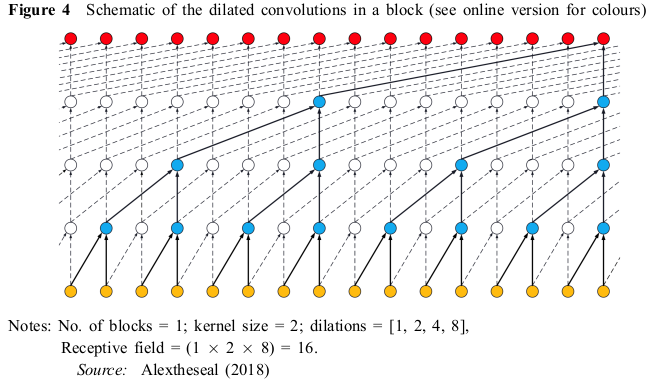
\includegraphics{img/2023-01-12-11-17-38.png}
  \end{itemize}
\item
  Disentangled-VAE:

  \begin{itemize}
  \item
    just a normal VAE with a value of \(\beta\) higher than one in the
    cost function (?):

    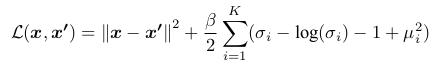
\includegraphics{img/2023-01-12-11-23-14.png}
  \item
    \begin{quote}
    Tuning the hyper-parameter β, to a value larger than one, can enable
    the factors to disentangle such that each coding only represents one
    factor at a time. Thus, greater interpretability of the model can be
    obtained. As such, the disentangled-VAE is also called a β-VAE
    \end{quote}
  \end{itemize}
\item
  \textbf{Latent space anomaly detection}: detect anomaly in the latent
  variables, i.e.~out-of-distribution. Several methods available.
  KL-divergence.
\item
  Datasets:

  \begin{itemize}
  \tightlist
  \item
    UC Berkeley Milling dataset. Freely available, small.
  \item
    Actual data from industry partener: 27 days, 5600 parts, annotated.
    Unavailable, large.
  \end{itemize}
\item
  Process:

  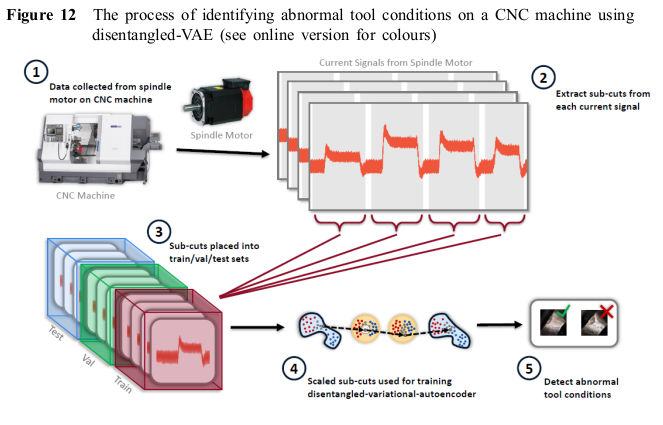
\includegraphics{img/2023-01-12-11-29-43.png}

  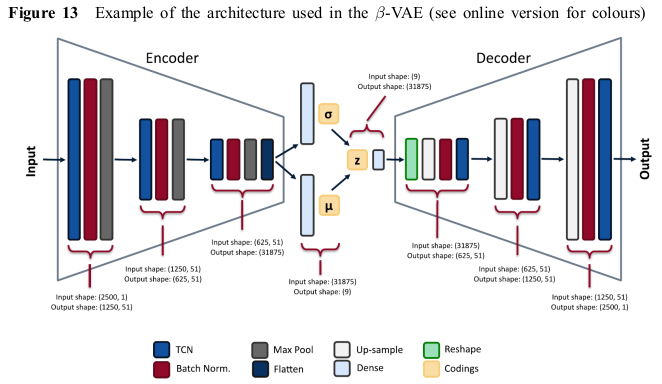
\includegraphics{img/2023-01-12-11-35-37.png}
\item
  Preprocessing:

  \begin{itemize}
  \tightlist
  \item
    select middle part of recording (stable cutting)
  \item
    sliding window
  \item
    MinMax scaling to \([0,1]\)
  \item
    each window labeled by hand (healthy / degraded / failed)
  \item
    randomly group windows into train/test sets
  \end{itemize}
\item
  Standard training
\item
  Results:

  \begin{itemize}
  \item
    PR-AUC 50\% for failed vs non-failed on the UC Berkeley dataset
    (PR-AUC = Precision-Recall AUC)

    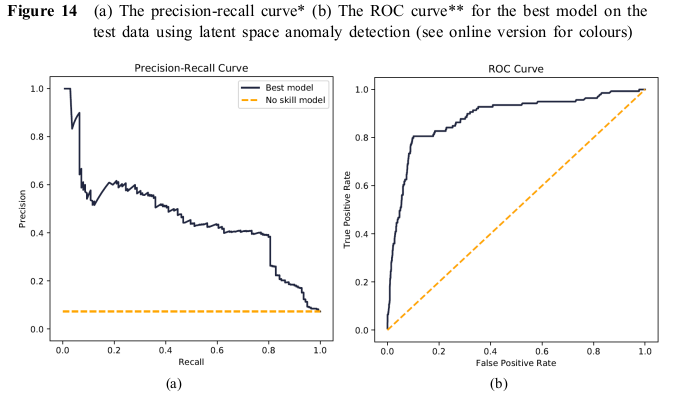
\includegraphics{img/2023-01-12-11-44-23.png}
  \item
    4\% PR-AUC on the industrial dataset ????!!!!

    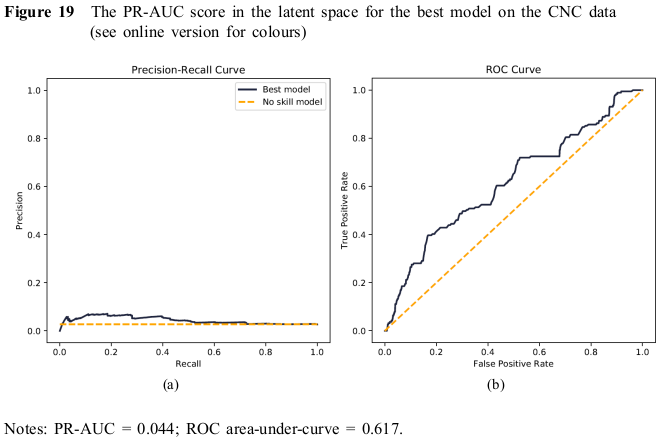
\includegraphics{img/2023-01-12-11-45-14.png}
  \end{itemize}
\end{itemize}

\begin{center}\rule{0.5\linewidth}{0.5pt}\end{center}

\hypertarget{mey2020}{%
\subsubsection{Mey2020}\label{mey2020}}

\begin{quote}
InProceedings (Mey2020)\\
Mey, O.; Neudeck, W.; Schneider, A. \& Enge-Rosenblatt, O.\\
Machine Learning-Based Unbalance Detection of a Rotating Shaft Using
Vibration Data\\
2020 25th IEEE International Conference on Emerging Technologies and
Factory Automation (ETFA), 2020, 1, 1610-1617
\end{quote}

\begin{itemize}
\tightlist
\item
  From
  \href{https://paperswithcode.com/paper/machine-learning-based-unbalance-detection-of}{PapersWithCode}
\item
  Code available in Github
  \href{https://github.com/deepinsights-analytica/ieee-etfa2020-paper}{here}
\item
  Uses (introduces) Fraunhoffer unbalance dataset
\end{itemize}

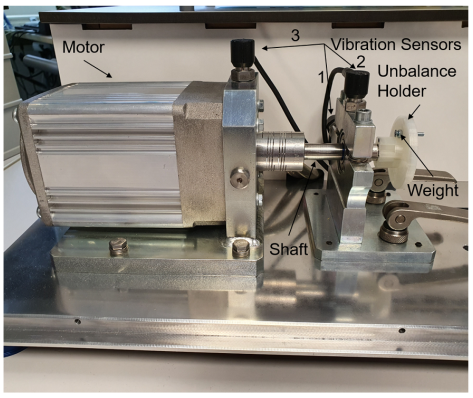
\includegraphics{img/2023-01-29-17-20-58.png}

\begin{itemize}
\item
  Goal: try do detect if unbalance is present on the rotating shaft
\item
  Introduces a new dataset (Fraunhoffer unbalance dataset)
\item
  Methods:
\item
  CNN on raw sensor data (windowed), 2-4 convs

  \begin{itemize}
  \tightlist
  \item
    90\% accuracy, weaker for small unbalance and particualar speeds
    (resonances?)
  \end{itemize}
\item
  Fully-connected MLP in FFT data

  \begin{itemize}
  \tightlist
  \item
    similar to CNN results
  \end{itemize}
\item
  Random Forests on automatically extracted timeseries features (again
  with \textbf{tsfresh})

  \begin{itemize}
  \tightlist
  \item
    similar (?)
  \end{itemize}
\item
  Hidden Markov Models on MFCC
\end{itemize}

Conclusions:

\begin{quote}
\begin{itemize}
\tightlist
\item
  The largest unbalance could be detected by all algorithms with almost
  perfect prediction accuracy, even if only 3 characteristic values per
  sample were used for the classification.
\item
  With the smaller unbalances, on the other hand, wider variations
  between the different approaches were found.
\item
  The best way to classify the dataset was to use an FC network with two
  hidden layers, which received the scaled FFT-transformed vibration
  data as input.
\item
  Measured on the entire evaluation dataset, 98.6 \% of the cases could
  be classified correctly.
\end{itemize}
\end{quote}

\hypertarget{datasets}{%
\subsection{Datasets}\label{datasets}}

\hypertarget{crwu-bearing-dataset}{%
\subsubsection{CRWU Bearing Dataset}\label{crwu-bearing-dataset}}

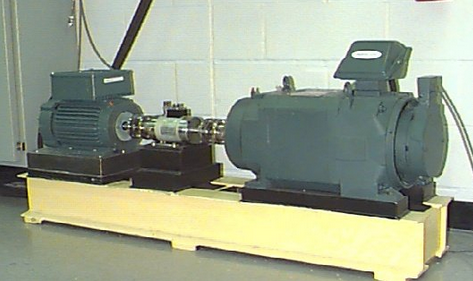
\includegraphics{img/2023-01-08-19-36-39.png}

\begin{itemize}
\tightlist
\item
  \href{https://engineering.case.edu/bearingdatacenter/download-data-file}{Link
  here}
\end{itemize}

\begin{quote}
Vibration data was collected using accelerometers, which were attached
to the housing with magnetic bases. Accelerometers were placed at the 12
o'clock position at both the drive end and fan end of the motor housing.
During some experiments, an accelerometer was attached to the motor
supporting base plate as well. Vibration signals were collected using a
16 channel DAT recorder, and were post processed in a Matlab
environment. All data files are in Matlab (*.mat) format. Digital data
was collected at 12,000 samples per second, and data was also collected
at 48,000 samples per second for drive end bearing faults. Speed and
horsepower data were collected using the torque transducer/encoder and
were recorded by hand.
\end{quote}

\begin{center}\rule{0.5\linewidth}{0.5pt}\end{center}

\hypertarget{uc-berkeley-milling-dataset-nasa}{%
\subsubsection{UC Berkeley Milling dataset,
NASA}\label{uc-berkeley-milling-dataset-nasa}}

\begin{itemize}
\tightlist
\item
  \href{https://www.nasa.gov/content/prognostics-center-of-excellence-data-set-repository}{Link
  here}
\item
  PapersWithCode:
  \href{https://paperswithcode.com/dataset/milling-data-set}{Link here}
\item
  Kaggle:
  \href{https://www.kaggle.com/datasets/vinayak123tyagi/milling-data-set-prognostic-data}{Link
  here}
\end{itemize}

\begin{quote}
Experiments on a milling machine for different speeds, feeds, and depth
of cut. Records the wear of the milling insert, VB. The data set was
provided by the UC Berkeley Emergent Space Tensegrities (BEST) Lab.
\end{quote}

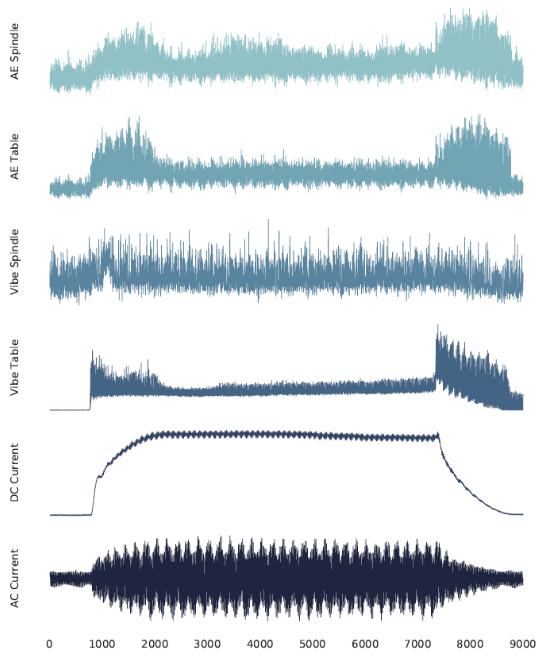
\includegraphics{img/2023-01-12-11-28-23.png}

\begin{center}\rule{0.5\linewidth}{0.5pt}\end{center}

\hypertarget{bosch-cnc-dataset}{%
\subsubsection{Bosch CNC dataset}\label{bosch-cnc-dataset}}

\begin{itemize}
\item
  \href{https://github.com/boschresearch/CNC_Machining}{Link here}
\item
  PapersWithCode:
  \href{https://paperswithcode.com/dataset/bosch-cnc-machining-dataset}{Link
  here}
\item
  Described in:

  \begin{quote}
  Article (Tnani2022)\\
  Tnani, M.-A.; Feil, M. \& Diepold, K.\\
  Smart Data Collection System for Brownfield CNC Milling Machines: A
  New Benchmark Dataset for Data-Driven Machine Monitoring\\
  Procedia CIRP, 2022, 107, 131-136
  \end{quote}
\item
  brownfield deployment: new hardware or software that must coexist with
  legacy IT systems
\item
  A whole procedure for collecting data and analyzing on the fly

  \begin{figure}

  {\centering 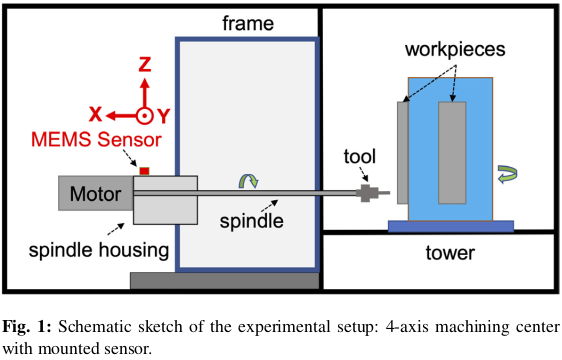
\includegraphics{img/2023-01-29-16-21-13.png}

  }

  \caption{Sensor mounting}

  \end{figure}

  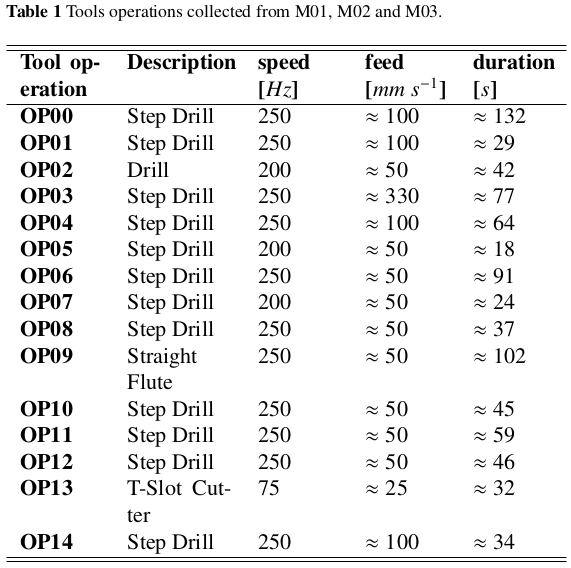
\includegraphics{img/2023-01-29-16-26-15.png}

  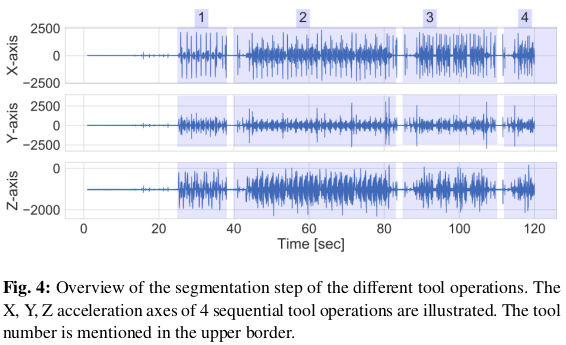
\includegraphics{img/2023-01-29-16-27-04.png}
\item
  Dataset:

  \begin{itemize}
  \tightlist
  \item
    vibration data collected with accelerometer sensors mounted to the
    rear end of the spindle housing
  \item
    collected over 2 years
  \item
    three diferent machines
  \item
    sampling rate 2 kHz, argue that it is enough for anomalies
  \item
    smart mining system, otherwise would need 4GB data per day
  \item
    15 different operations recorded, with different parameterizations
  \item
    labeled \textbf{good vs bad} (normal vs anomaly)
  \end{itemize}
\item
  Processing:

  \begin{itemize}
  \tightlist
  \item
    \textbf{Tsfresh}: automatic package to extract standard features
    from time series, open source,
    \href{https://tsfresh.readthedocs.io/en/latest/}{here},
    \href{https://www.sciencedirect.com/science/article/pii/S0925231218304843}{paper
    here}
  \end{itemize}
\item
  Real world challenges:

  \begin{itemize}
  \tightlist
  \item
    problems when changing tools =\textgreater{} some recordings are bad
  \item
    unbalanced data (815 to 35)
  \item
    normal wear of tools, hydraulic issues, incorrect settings
    =\textgreater{} some variability
  \item
    15 different operations recorded, with different parameterizations
    =\textgreater{} \textbf{difficult to predict health status, it
    depends on all params}

    \begin{itemize}
    \item
      \begin{quote}
      anomaly can be detected in frequencies which are integer multiples
      of the spindle speed ()
      \end{quote}
    \item
      anomalies better detected in frequency domain
    \end{itemize}
  \end{itemize}
\end{itemize}

\hypertarget{ims-bearing-dataset-cincinatti-nasa}{%
\subsubsection{IMS Bearing Dataset, Cincinatti,
NASA}\label{ims-bearing-dataset-cincinatti-nasa}}

\begin{itemize}
\item
  \href{https://www.nasa.gov/content/prognostics-center-of-excellence-data-set-repository}{Link
  here}, no.4
\item
  PapersWithCode:
  \href{https://paperswithcode.com/dataset/ims-bearing-dataset}{Link
  here}
\item
  Kaggle:
  \href{https://www.kaggle.com/datasets/vinayak123tyagi/bearing-dataset}{Link
  here}
\item
  Accelerometer data in turning bearings, recorded until they fail
\end{itemize}

\begin{quote}
Four bearings were installed on a shaft. The rotation speed was kept
constant at 2000 RPM by an AC motor coupled to the shaft via rub belts.
A radial load of 6000 lbs is applied onto the shaft \textgreater{} and
bearing by a spring mechanism. All bearings are force lubricated.
Rexnord ZA-2115 double row bearings were installed on the shaft as shown
in Figure 1. PCB 353B33 High Sensitivity Quartz ICP accelerometers were
installed on the bearing housing (two accelerometers for each bearing
{[}x- and y-axes{]} for data set 1, one accelerometer for each bearing
for data sets 2 and 3). Sensor placement is also shown in Figure 1. All
failures occurred after exceeding designed life time of the bearing
which is more than 100 million revolutions.
\end{quote}

\hypertarget{fraunhoffer-unbalance-dataset}{%
\subsubsection{Fraunhoffer unbalance
dataset}\label{fraunhoffer-unbalance-dataset}}

\begin{itemize}
\item
  \href{https://fordatis.fraunhofer.de/handle/fordatis/151.3}{Link here}
\item
  PapersWithCode:
  \href{https://paperswithcode.com/dataset/unbalance-classification-using-vibration-data}{Link
  here}
\item
  Kaggle:
  \href{https://www.kaggle.com/datasets/vinayak123tyagi/bearing-dataset}{Link
  here}
\item
  Used by (Mey et al. 2020)
\item
  Not CNC
\item
  A vibrating drive train (DC motor, shaft roller bearing)
\item
  Unbalances of different weights and radii are attached to the shaft
\end{itemize}

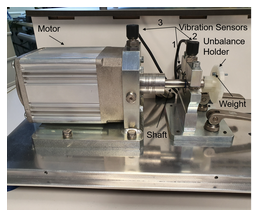
\includegraphics{img/2023-01-29-17-13-53.png}

\begin{quote}
This dataset contains vibration data recorded on a rotating drive train.
This drive train consists of an electronically commutated DC motor and a
shaft driven by it, which passes through a roller bearing. With the help
of a 3D-printed holder, unbalances with different weights and different
radii were attached to the shaft. Besides the strength of the
unbalances, the rotation speed of the motor was also varied. This
dataset can be used to develop and test algorithms for the automatic
detection of unbalances on drive trains. Datasets for 4 differently
sized unbalances and for the unbalance-free case were recorded. The
vibration data was recorded at a sampling rate of 4096 values per
second. Datasets for development (ID ``D{[}0-4{]}'') as well as for
evaluation (ID ``E{[}0-4{]}'') are available for each unbalance
strength. The rotation speed was varied between approx. 630 and 2330 RPM
in the development datasets and between approx. 1060 and 1900 RPM in the
evaluation datasets. For each measurement of the development dataset
there are approx. 107min of continuous measurement data available, for
each measurement of the evaluation dataset 28min. Details of the
recorded measurements and the used unbalance strengths are documented in
the README.md file
\end{quote}

\begin{itemize}
\item
  Each csv file contains:

  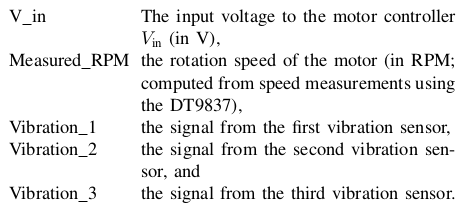
\includegraphics{img/2023-01-29-17-22-33.png}
\end{itemize}

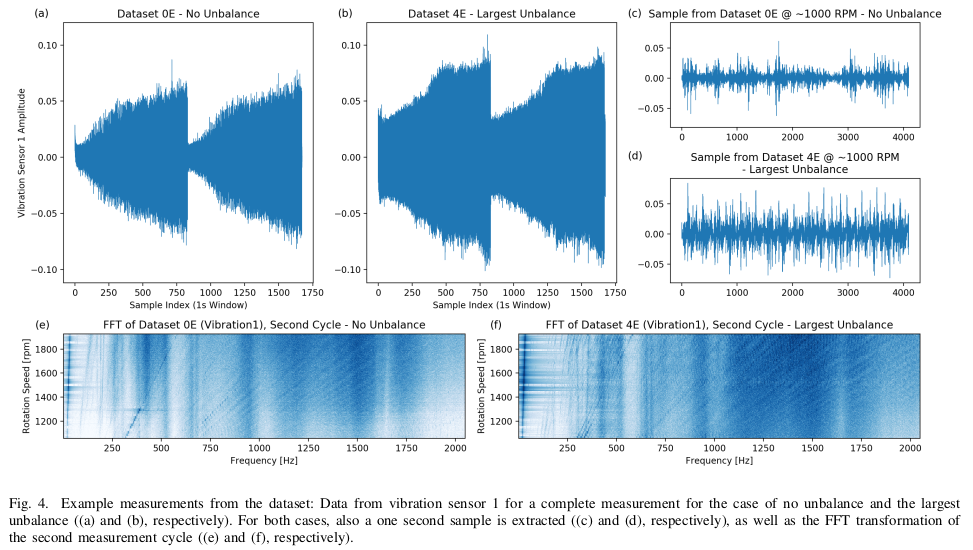
\includegraphics{img/2023-01-29-17-23-08.png}

\hypertarget{refs}{}
\begin{CSLReferences}{1}{0}
\leavevmode\vadjust pre{\hypertarget{ref-Cho2005}{}}%
Cho, Sohyung, Shihab Asfour, Arzu Onar, and Nandita Kaundinya. 2005.
{``Tool Breakage Detection Using Support Vector Machine Learning in a
Milling Process.''} \emph{International Journal of Machine Tools and
Manufacture} 45 (3): 241--49.
\url{https://doi.org/10.1016/j.ijmachtools.2004.08.016}.

\leavevmode\vadjust pre{\hypertarget{ref-Ordas2017_WearCharactPhD}{}}%
García-Ordás, Teresa María. 2017. {``Wear Characterization of the
Cutting Tool in Milling Processes Using Shape and Texture
Descriptors.''} PhD thesis. \url{https://doi.org/10.18002/10612/6915}.

\leavevmode\vadjust pre{\hypertarget{ref-Kankar2011}{}}%
Kankar, P. K., Satish C. Sharma, and S. P. Harsha. 2011. {``Fault
Diagnosis of Ball Bearings Using Machine Learning Methods.''}
\emph{Expert Systems with Applications} 38 (3): 1876--86.
\url{https://doi.org/10.1016/j.eswa.2010.07.119}.

\leavevmode\vadjust pre{\hypertarget{ref-Kim2018_SmartMachineReview}{}}%
Kim, Dong-Hyeon, Thomas J. Y. Kim, Xinlin Wang, Mincheol Kim, Ying-Jun
Quan, Jin Woo Oh, Soo-Hong Min, et al. 2018. {``Smart Machining Process
Using Machine Learning: A Review and Perspective on Machining
Industry.''} \emph{International Journal of Precision Engineering and
Manufacturing-Green Technology} 5 (4): 555--68.
\url{https://doi.org/10.1007/s40684-018-0057-y}.

\leavevmode\vadjust pre{\hypertarget{ref-Li2017}{}}%
Li, Shaobo, Guokai Liu, Xianghong Tang, Jianguang Lu, and Jianjun Hu.
2017. {``An {Ensemble} {Deep} {Convolutional} {Neural} {Network} {Model}
with {Improved} {D}-{S} {Evidence} {Fusion} for {Bearing} {Fault}
{Diagnosis}.''} \emph{Sensors} 17 (8): 1729.
\url{https://doi.org/10.3390/s17081729}.

\leavevmode\vadjust pre{\hypertarget{ref-Mey2020}{}}%
Mey, Oliver, Willi Neudeck, André Schneider, and Olaf Enge-Rosenblatt.
2020. {``Machine {Learning}-{Based} {Unbalance} {Detection} of a
{Rotating} {Shaft} {Using} {Vibration} {Data}.''} In \emph{2020 25th
{IEEE} {International} {Conference} on {Emerging} {Technologies} and
{Factory} {Automation} ({ETFA})}, 1:1610--17.
\url{https://doi.org/10.1109/ETFA46521.2020.9212000}.

\leavevmode\vadjust pre{\hypertarget{ref-Ong2019}{}}%
Ong, Pauline, Woon Kiow Lee, and Raymond Jit Hoo Lau. 2019. {``Tool
Condition Monitoring in {CNC} End Milling Using Wavelet Neural Network
Based on Machine Vision.''} \emph{The International Journal of Advanced
Manufacturing Technology} 104 (1): 1369--79.
\url{https://doi.org/10.1007/s00170-019-04020-6}.

\leavevmode\vadjust pre{\hypertarget{ref-Papandrea2020}{}}%
Papandrea, Pedro J., Edielson P. Frigieri, Paulo Roberto Maia, Lucas G.
Oliveira, and Anderson P. Paiva. 2020. {``Surface Roughness Diagnosis in
Hard Turning Using Acoustic Signals and Support Vector Machine: {A}
{PCA}-Based Approach.''} \emph{Applied Acoustics} 159 (February):
107102. \url{https://doi.org/10.1016/j.apacoust.2019.107102}.

\leavevmode\vadjust pre{\hypertarget{ref-Tambake2021}{}}%
Tambake, Nagesh R., Bhagyesh B. Deshmukh, and Abhishek D. Patange. 2021.
{``Data {Driven} {Cutting} {Tool} {Fault} {Diagnosis} {System} {Using}
{Machine} {Learning} {Approach}: {A} {Review}.''} \emph{Journal of
Physics: Conference Series} 1969 (1): 012049.
\url{https://doi.org/10.1088/1742-6596/1969/1/012049}.

\end{CSLReferences}



\end{document}
